\section{Contexte}
En l'état actuel, lorsque les pompiers doivent intervenir dans le cas d'un incident impliquant des fuites d'hydrocarbures sur route, la répartition
du produit absorbant se fait via une remorque-semoirs.Celle-ci dispose de trois sections de dépose du produit sont télécommandées directement par un opérateur.
Durant l'intervention, une personne doit marcher à côté de la remorque afin d'observer et contrôler la répartition du produit, nous pouvons relever les points suivant:
\begin{enumerate}
    \item L'opérateur doit marcher, cela limite la vitesse du véhicule et les longues distances sont problématiques.
    \item La détection se fait à l'oeil nu, l'opérateur doit donc rester concentrer en permanence au risque de devoir repasser sur certaines zone.
    \item La commande est manuelle, il est possible de faire des erreurs d'erreur sur la commande risquant la dépose de surplus de produit ou de devoir repasser sur certaines zone.
\end{enumerate}
\textbf{Le but de se travail de Bachelor est d'automatiser ce processus, via un système de détection des hydrocarbures par vision industrielle et d'un pilotage de l'ouverture/fermeture des vérins.}
\section{Cahier des charges \label{cdc}}
Le cahier des charges est le suivant:
\begin{itemize}
    \item Préparer un planning détaillant les tâches.
    \item Définir un setup permettant de:
          \begin{itemize}
              \item Analyser les traces d'hydrocarbures selon leur positionnement sur la route.
              \item Commander la télécommande du semoir.
          \end{itemize}
    \item Sélectionner les éléments composant le setup.
    \item Commander les éléments.
    \item Assembler les éléments.
    \item Tester le setup et procéder aux ajustements nécessaires.
    \item Développer un logiciel d'analyse et de gestion de la télécommande.
    \item Tester le logiciel d'analyse et de gestion de la télécommande.
    \item Valider le logiciel et le comportement sur la route.
    \item Analyser et interpréter les résultats.
\end{itemize}
\section{Planning}
Le planning vient compléter le cahier des charges du chapitre \ref{cdc} en ajoutant le travail à effectuer pour chaque étape ainsi qu'une estimation
de l'effort à fournir en heure.

Le planning ci-dessous présente les étapes, le détail des sous-étapes, l'effort à fournir estimé ainsi que la période durant laquelle chaque étape seront présumément effectuée (en bleu).
\begin{figure}[H]
    \centering
    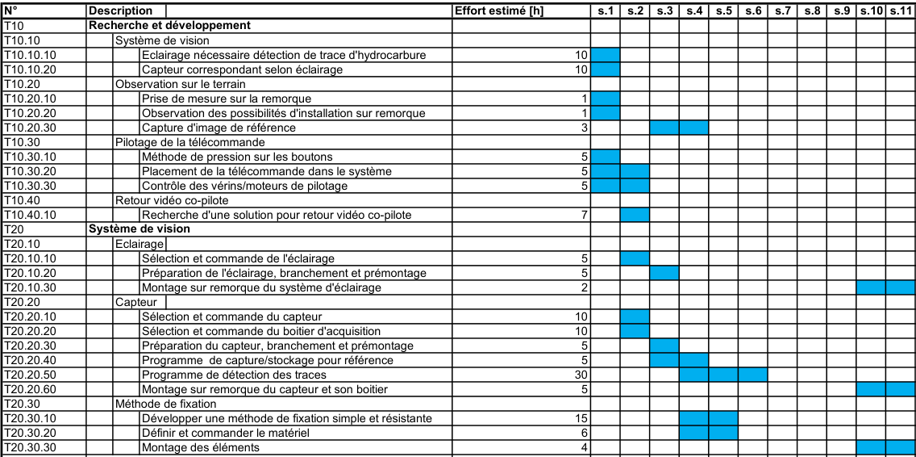
\includegraphics[width=15cm, angle=90]{assets/figures/planning1.png}
    \caption{Planning - partie 1}
\end{figure}
\newpage
\begin{figure}[H]
    \centering
    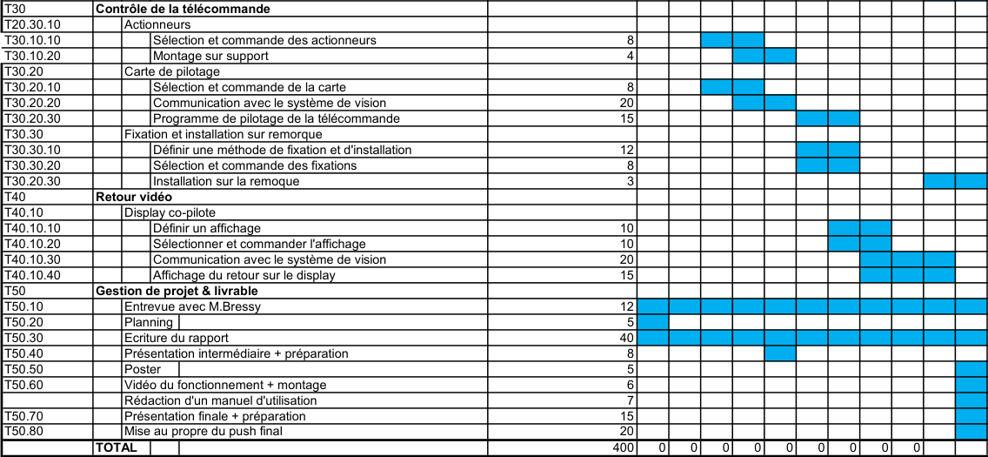
\includegraphics[width=15cm, angle=90]{assets/figures/planning2.png}
    \caption{Planning - partie 2}
\end{figure}

En complément au planning ci-dessus, on peut imaginer une vingtaine d'heures d'imprévus supplémentaires.
\iffalse
    %%if
    \section{Citations et bibliographie}
    Citer vos sources est essentiel. Avec \texttt{biblatex} vous pouvez facilement citer des articles, des livres ou des sites internet. Toutes les citations dans le texte seront automatiquement regroupées en fin de document dans la section \guillemotleft Bibliographie\guillemotright. Par exemple, citons un article d'Einstein \cite{einstein} ou le livre de Dirac \cite{dirac}.
    
    Parfois il peut être utile d'utiliser un gestionnaire de bibliographie. La communauté académique recommande l'outil \href{https://www.zotero.org/}{Zotero} qui permet de gérer une bibliothèque numérique d'ouvrages et de références numériques. Il permet également de générer une bibliographie compatible avec \LaTeX.
    
    Notez qu'il est très facile d'obtenir l'extrait \texttt{bibtex} depuis des journaux. Sélectionnez \emph{export/citation}. Si vous le pouvez choisissez \texttt{bibtex}. Dans le cas d'un format \texttt{.ris}, utilisez un convertisseur en ligne comme \href{http://www.bruot.org/ris2bib/}{ris2bib}.
    
    \section{Adapter votre modèle}
    Ce document n'est qu'un modèle ayant pour but de revoir les quelques avantages de \LaTeX~ et les fonctionnalités qui pourraient vous être utiles pour rédiger un rapport académique. N'hésitez pas à supprimer les parties inutiles et à adapter ce modèle à vos besoins.
    %%fi
\fi